\chapter{\sffamily Multi-agent markets}

{\bfseries\sffamily Concept.} The idea here is 

\begin{figure}[h]
\centering
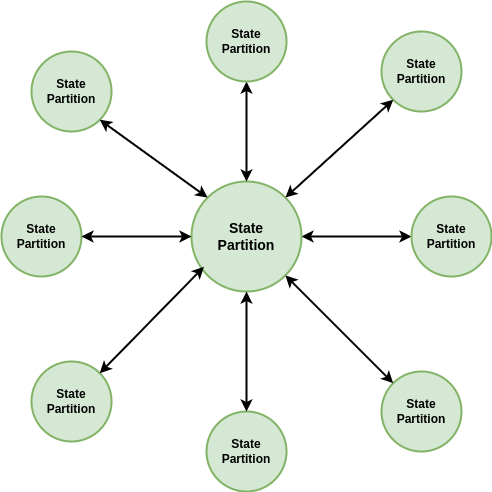
\includegraphics[width=9cm]{images/chapter-10-state-partition-graph.drawio.png}
\caption{State partition graph topology for multi-agent market archetypes.}
\label{fig:state-partition-graph-multi-agent-markets}
\end{figure}

\textcolor{red}{
\begin{itemize}
\item{Full sim: full event-based spatial stochastic model}
\item{Inference model: spatial mean field inference features using the probabilistic reweighting }
\item{Also use the likelihood-free inference model?}
\end{itemize}
}

\textcolor{red}{
\begin{itemize}
\item{Humanitarian aid logistics in response to flooding, fire or other natural disasters}
\item{Routing of transportation}
\item{Where to focus searches}
\item{Transportation size distribution}
\item{Supply chain logistics of resources and allocation of budget}
\item{Example paper here with stochastic network models~\cite{alem2016stochastic}}
\end{itemize}
}